\documentclass[UTF8]{ctexart}
\usepackage{listings}
\usepackage{textcomp} % 必须加上,否则报错
\usepackage{xcolor}
\usepackage{amsmath}
\pagestyle{plain}
\usepackage{fontspec}
\usepackage{graphicx}  
\usepackage{epstopdf}
\CTEXsetup[format={\Large\bfseries}]{section}
\lstset{language=Matlab}%代码语言使用的是matlab
\lstset{breaklines}%自动将长的代码行换行排版
\lstset{extendedchars=false}%解决代码跨页时,章节标题,页眉等汉字不显示的问题
\CTEXoptions[today=old] 
\title{Assignment 2}  %文章标题
\author{Zou Yuan\\Student No. 21960216}   %作者的名称
\date{\today}       %日期
\begin{document}
	\maketitle
	\section{Jacobi Method}
	The problems to be solved in this section are below:
	
	Use the Jacobi Method to solve the sparse system within three correct decimal places (forward
	error in the infinity norm) for $n = 100$. The correct solution is $[1,−1,1,−1, \dots ,1,−1]$. Report
	the number of steps needed and the backward error. The system is

	$$
	\begin{bmatrix} 
		2  &1 &    \\1 &2  &1&   \\&\ddots &\ddots&\ddots\\& &1  &2 &1\\ & & &1&2
	\end{bmatrix}\begin{bmatrix}x_1\\ \\\vdots\\ \\x_n\end{bmatrix}=\begin{bmatrix}
	1    \\0  \\\vdots  \\0\\-1
	\end{bmatrix}$$
	
	The Matlab code is as follows:
	
	\begin{centering}
	\begin{lstlisting}
	n=100;
	[a,b]=sparsesetup(n);
	[x,cout]=jacobi(a,b)
	
	function [a,b] = sparsesetup(n)
	e = ones(n,1);
	n2=n/2;
	a = spdiags([e 2*e e],-1:1,n,n);   
	b=zeros(n,1);                         
	b(1)=1;b(n)=-1;
	end
	
	
	function [x2,cout]=jacobi(B,c)
	
	D=diag(diag(B));
	U=D-triu(B);
	L=D-(triu(B))';
	x1=(rand(1,size(B,1)))';
	cout=0;
	while 1
	cout=cout+1;
	x2=inv(D)*(U+L)*x1+inv(D)*c;
	t=ones(1,size(B,1));
	t(2:2:size(B,1))=-1;
	t=t';
	t1=x2-x1;
	t2=x2-t;
	if (norm(t1,inf)<10e-3)&&(norm(t2,inf)<10e-3)
	break
	end
	x1=x2;
	end
	
	end
	\end{lstlisting}
		\end{centering}
	
The output is:
\begin{align*}
\begin{split}
&cout =10896\\
&back \underline{\hspace{0.5em}}error =0.0137
\end{split}
\end{align*}

As shown above, the number of iterations is 10896 which varies slightly with the initial value, and the backward error is 0.0137.
\section{Gauss–Seidel  Method}
   This chapter uses the Gauss–Seidel method method and the SOR method to solve the problems in the previous chapter.
   
Gauss–Seidel method:
   \begin{centering}
   	\begin{lstlisting}
   	n=100;
   	[a,b]=sparsesetup(n);
   	x1=(rand(1,n))';
   	[x,cout]=seidel(a,b)
   	back_error=norm(b-a*x,inf)
   	
   	function [a,b] = sparsesetup(n)
   	e = ones(n,1);
   	n2=n/2;
   	a = spdiags([e 2*e e],-1:1,n,n);    
   	b=zeros(n,1);                         
   	b(1)=1;b(n)=-1;
   	end
   	function [x2,cout]=seidel(A,b)
   	
   	D=diag(diag(A));
   	L = -tril(A,-1);%求A的下三角矩阵
   	U = -triu(A,1);%求A的上三角矩阵
   	G = (D-L)\U;
   	f = (D-L)\b;
   	x0=(rand(1,size(A,1)))';
   	x = G*x0+f;
   	cout=0;  %迭代次数
   	t=ones(1,size(A,1));
   	t(2:2:size(A,1))=-1;
   	t=t';
   	while 1
   	x0 = x;
   	x = G*x0+f;
   	cout = cout+1;
   	if (norm(x-x0,inf)<10e-3)&&(norm(x-t,inf)<10e-3)
   	break
   	end
   	x2=x;
   	end
   	
   	end
   	
   	\end{lstlisting}   \end{centering}
   
 SOR method:
   \begin{centering}
   	\begin{lstlisting}
   	n=100;
   	[a,b]=sparsesetup(n);
   	x1=(rand(1,n))';
   	[x,cout]=seidel(a,b)
   	back_error=norm(b-a*x,inf)
   	
   	function [a,b] = sparsesetup(n)
   	e = ones(n,1);
   	n2=n/2;
   	a = spdiags([e 2*e e],-1:1,n,n);    
   	b=zeros(n,1);                        
   	b(1)=1;b(n)=-1;
   	end
   	function [x2,cout]=seidel(A,b)
   	
   	D=diag(diag(A));
   	L = -tril(A,-1);%求A的下三角矩阵
   	U = -triu(A,1);%求A的上三角矩阵
   	w=1.5;
   	G = (D-w*L)\((1-w)*D+w*U);
   	f = (D-w*L)\(w*b);
   	x0=(rand(1,size(A,1)))';
   	x = G*x0+f;
   	cout=0;  %迭代次数
   	t=ones(1,size(A,1));
   	t(2:2:size(A,1))=-1;
   	t=t';
   	while 1
   	x0 = x;
   	x = G*x0+f;
   	cout = cout+1;
   	if (norm(x-x0,inf)<10e-3)&&(norm(x-t,inf)<10e-3)
   	break
   	end
   	x2=x;
   	end
   	
   	end
   	\end{lstlisting}   \end{centering}

The Seidel method output is:
\begin{align*}
\begin{split}
&cout = 5031\\
&back \underline{\hspace{0.5em}}error =9.6863e-06
\end{split}
\end{align*}
The SOR output is:
\begin{align*}
\begin{split}
&cout = 1659\\
&back \underline{\hspace{0.5em}}error =9.7578e-06
\end{split}
\end{align*}

As shown above, These methods can converge faster and get Higher precision than Jacobi method.
\section{Cojugate Method}
The problems to be solved in this section are below:

Let A be the n × n matrix with n = 1000 and entries
$A(i, i) = i,A(i, i + 1) = A(i + 1, i) = 1/2,A(i, i + 2) = A(i + 2, i) = 1/2$ for all\quad $i$ that fit
within the matrix. (a) Print the nonzero structure spy(A). (b) Let $x_e$ be the vector of n ones.
Set $b = Ax_e$, and apply the Conjugate Gradient Method, without preconditioner, with the
Jacobi preconditioner, and with the Gauss–Seidel preconditioner. Compare errors of the three runs in a plot versus step number.
\begin{centering}
	\begin{lstlisting}	
	n=1000;
	[a,b]=matrixetup(n);
	xc=ones(n,1);
	[x1,cout1,be1]=conjugate(a,b);
	dd=diag(diag(a));
	a=dd\a;
	b=dd\b;
	[x2,cout2,be2]=jacobi(a,b,xc);
	[x3,cout3,be3]=guaseidel(a,b,xc);
	t=1:100;
	figure();
	plot(t,be1,'-o',t,be2,'-h',t,be3,'-s')
	semilogy(t,be1,'-o',t,be2,'-h',t,be3,'-s')
	legend('conjugate','Prejacobi','PregaussSeidel');
	
	
	function [a,b] = matrixetup(n)
	v=(1:1:n);
	a=diag(v);
	for i=1:n-2
	a(i,i+1)=1/2;a(i+1,i)=1/2;
	a(i,i+2)=1/2;a(i+2,i)=1/2;
	end
	xe=ones(n,1);                         
	b=a*xe;
	end
	
	function [x,t,be]=jacobi(a,c,xc)
	D=diag(diag(a));     
	U=D-triu(a);
	L=-tril(a,-1);
	for t=1:100
	x=inv(D)*(U+L)*xc+inv(D)*c; 
	be(t)=norm(x-xc,'inf');
	end
	end
	function [x,t,be] = guaseidel(a,b,xc)
	D=diag(diag(a));
	L = -tril(a,-1);
	U = -triu(a,1);
	G = (D-L)\U;
	f = (D-L)\b;
	x0=(rand(1,size(a,1)))';
	x = G*x0+f;
	for t=1:100
	be(t)=norm(x-xc,'inf');
	x0 = x;
	x = G*x0+f;
	end
	end
	function [x,t,be]=conjugate(a,b)
	n=length(b);
	xc=ones(n,1);
	x=zeros(n,1);
	r=b-a*x;
	d=r;
	for t=1:100
	G=(norm(r)^2)/(d'*a*d);
	x=x+G*d;
	rr=b-a*x;
	be(t)=norm(x-xc,'inf');
	B=(norm(rr)^2)/(norm(r)^2);
	d=rr+B*d;
	r=rr;
	end
	end
	
	\end{lstlisting}  
 \end{centering}

Result is below:
\begin{figure} [h]
	\centering  
	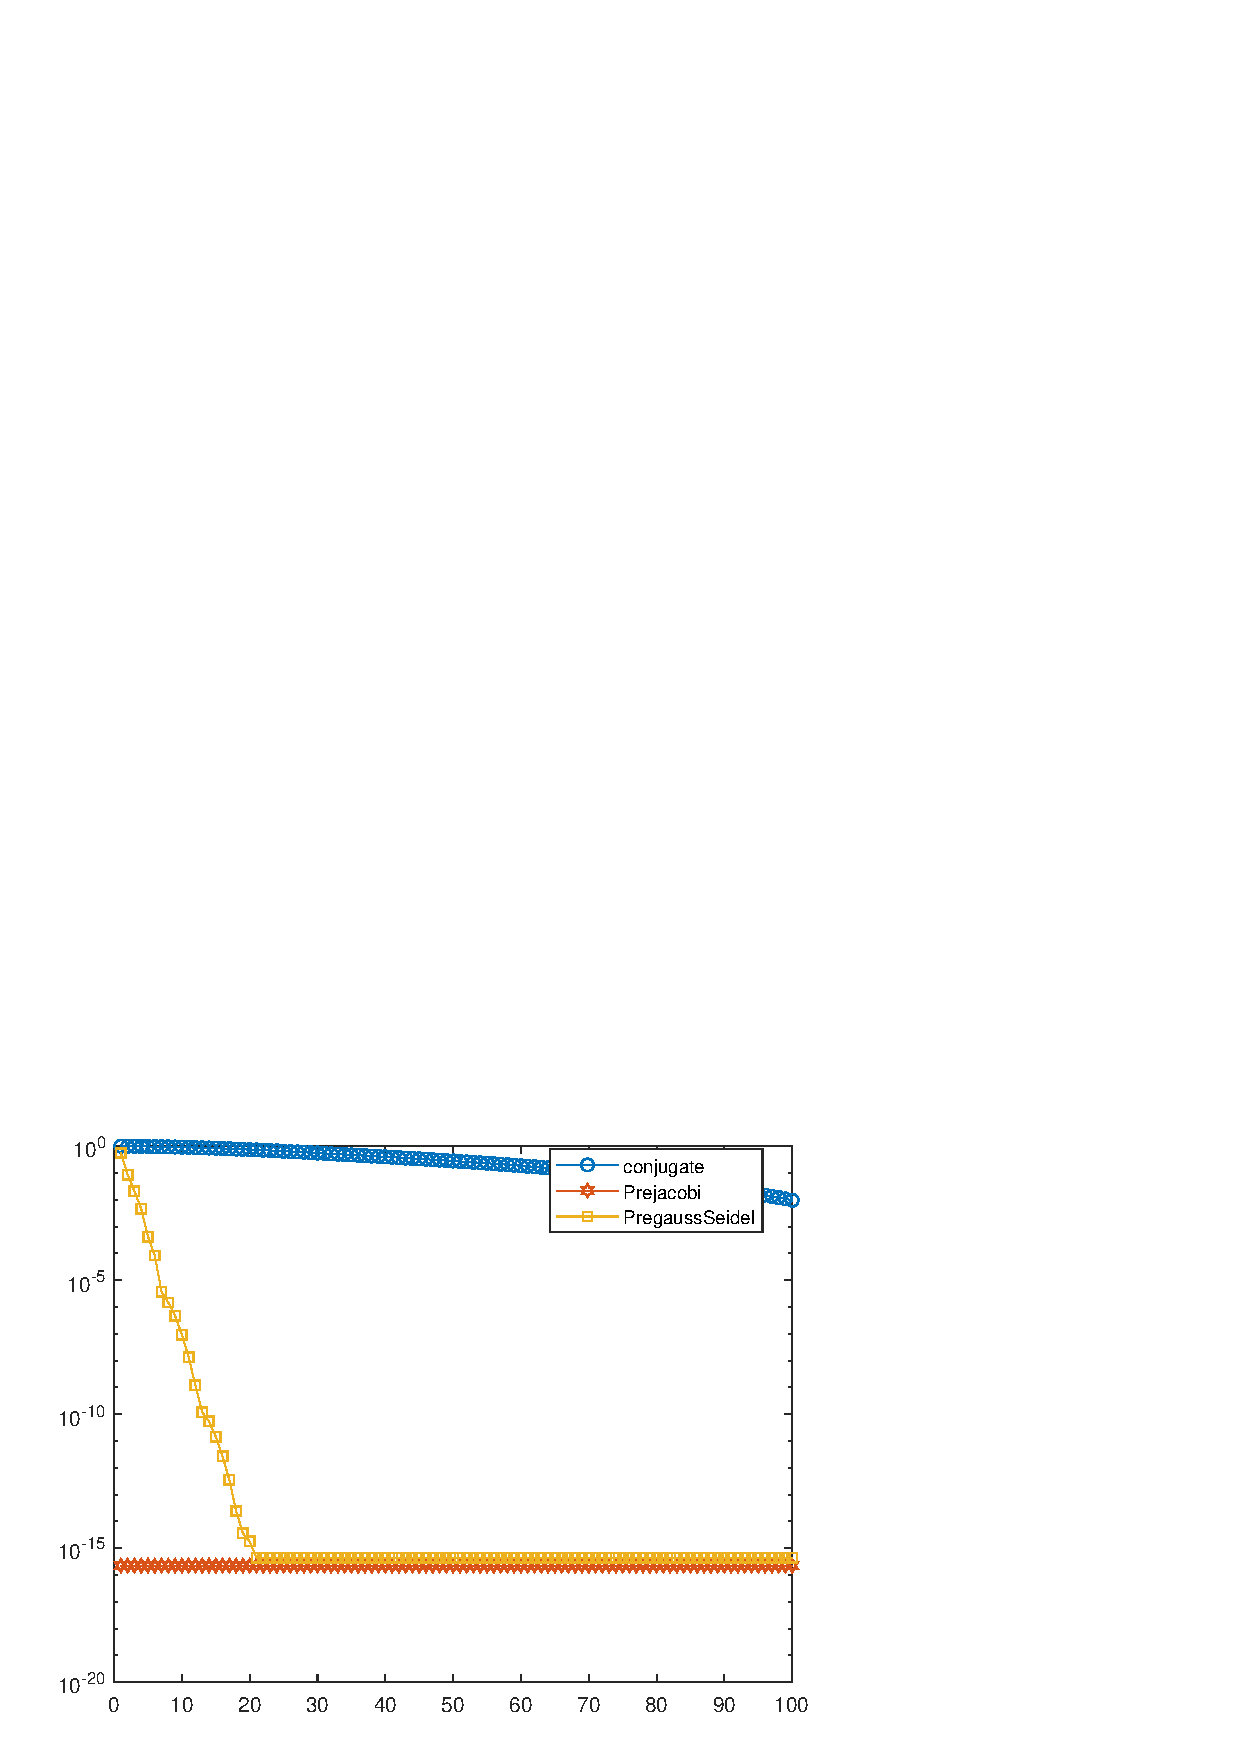
\includegraphics[scale=0.7]{1.jpg}  
	\caption{Converge Results}  
	\label{1}  
\end{figure}  
\end{document}
